\subsection{Optimisations and experimental evaluation}
\label{subsec:pureshift__dpsyche_optimisation}


\subsubsection{Spectrum-comparison cost function}

As previously discussed, the fact that the dPSYCHE experiment can be very quickly simulated opens up the potential for entirely computational optimisation of the pulse sequence.
For any arbitrary spin system, it is trivial to remove all the couplings \textit{in silico} and simulate a pulse--acquire spectrum: this gives us a theoretically perfect pure shift spectrum.
The simulated dPSYCHE experiment (on a system with couplings) can then be compared against this.
The entire process is repeated using $s$ different spin systems, and the cost function is defined as:
\begin{equation}
    \label{eq:f_diff_dpsyche}
    f_\text{diff,2} = \frac{1}{s}\sum_s \Biggl\lVert \frac{\symbf{S}_\text{re} - c\symbf{T}_\text{re}}{c\lVert \symbf{T}_\text{re} \rVert} \Biggr\rVert^2
\end{equation}
where $\symbf{S}$ is the dPSYCHE spectrum, and $\symbf{T}$ is the target spectrum.
The prefactor $c$ will be discussed later; for now I treat it as $1$.
This cost function appears superficially very similar to $f_\text{diff}$ (discussed in \cref{subsec:pureshift__optim_techniques}), and is based on the same principle that we want the spectra $\symbf{S}$ and $\symbf{T}$ to match one another, but there are several points of note:
\begin{itemize}
    \item The spectrum $\symbf{S}_\text{re}$ is not scaled down by its norm. This means that the sensitivity penalty no longer comes from the difference in the noise (as was previously the case), but rather directly from the difference in peak intensity.
        Since simulated spectra are noiseless, the original $f_\text{diff}$ would not work here.
    \item The division of the entire cost function by $\lVert\symbf{T}_\text{re}\rVert$ is not important if only one spin system is being simulated as it is simply a constant factor.
        However, if more than one spin system is being simulated, $\lVert\symbf{T}_\text{re}\rVert$ differs from system to system and this factor helps to essentially normalise the contributions from each spin system.
    \item The norm in the cost function here is squared.
        Again, this makes no difference to the optimum if only one spin system is being investigated, because $x^2$ is strictly increasing for $x > 0$.\footnote{It may affect the rate of convergence, but this is not something I tested.}
        However, for multiple spin systems it makes sense to square the norm, as the largest deviations will be penalised more greatly: this means that a pure shift spectrum which works reasonably well across a wide range of spin systems will be prioritised over one which works perfectly well for some and fails badly for others.
\end{itemize}

I began by first checking how many $t_1$ increments (i.e.\ chunks) were required in the simulation to obtain reliable cost function values.
If too few chunks are simulated, the resulting pure shift spectrum will have truncation artefacts, which are likely to mask artefacts from unwanted CTPs.
The value of $f_\text{diff,2}$ was thus tested with a wide variety of randomly chosen phases and angles, with the number of chunks set to 4, 8, and 16 (\cref{fig:dpsyche_td1_cf}).

\begin{figure}[htb]
    \centering
    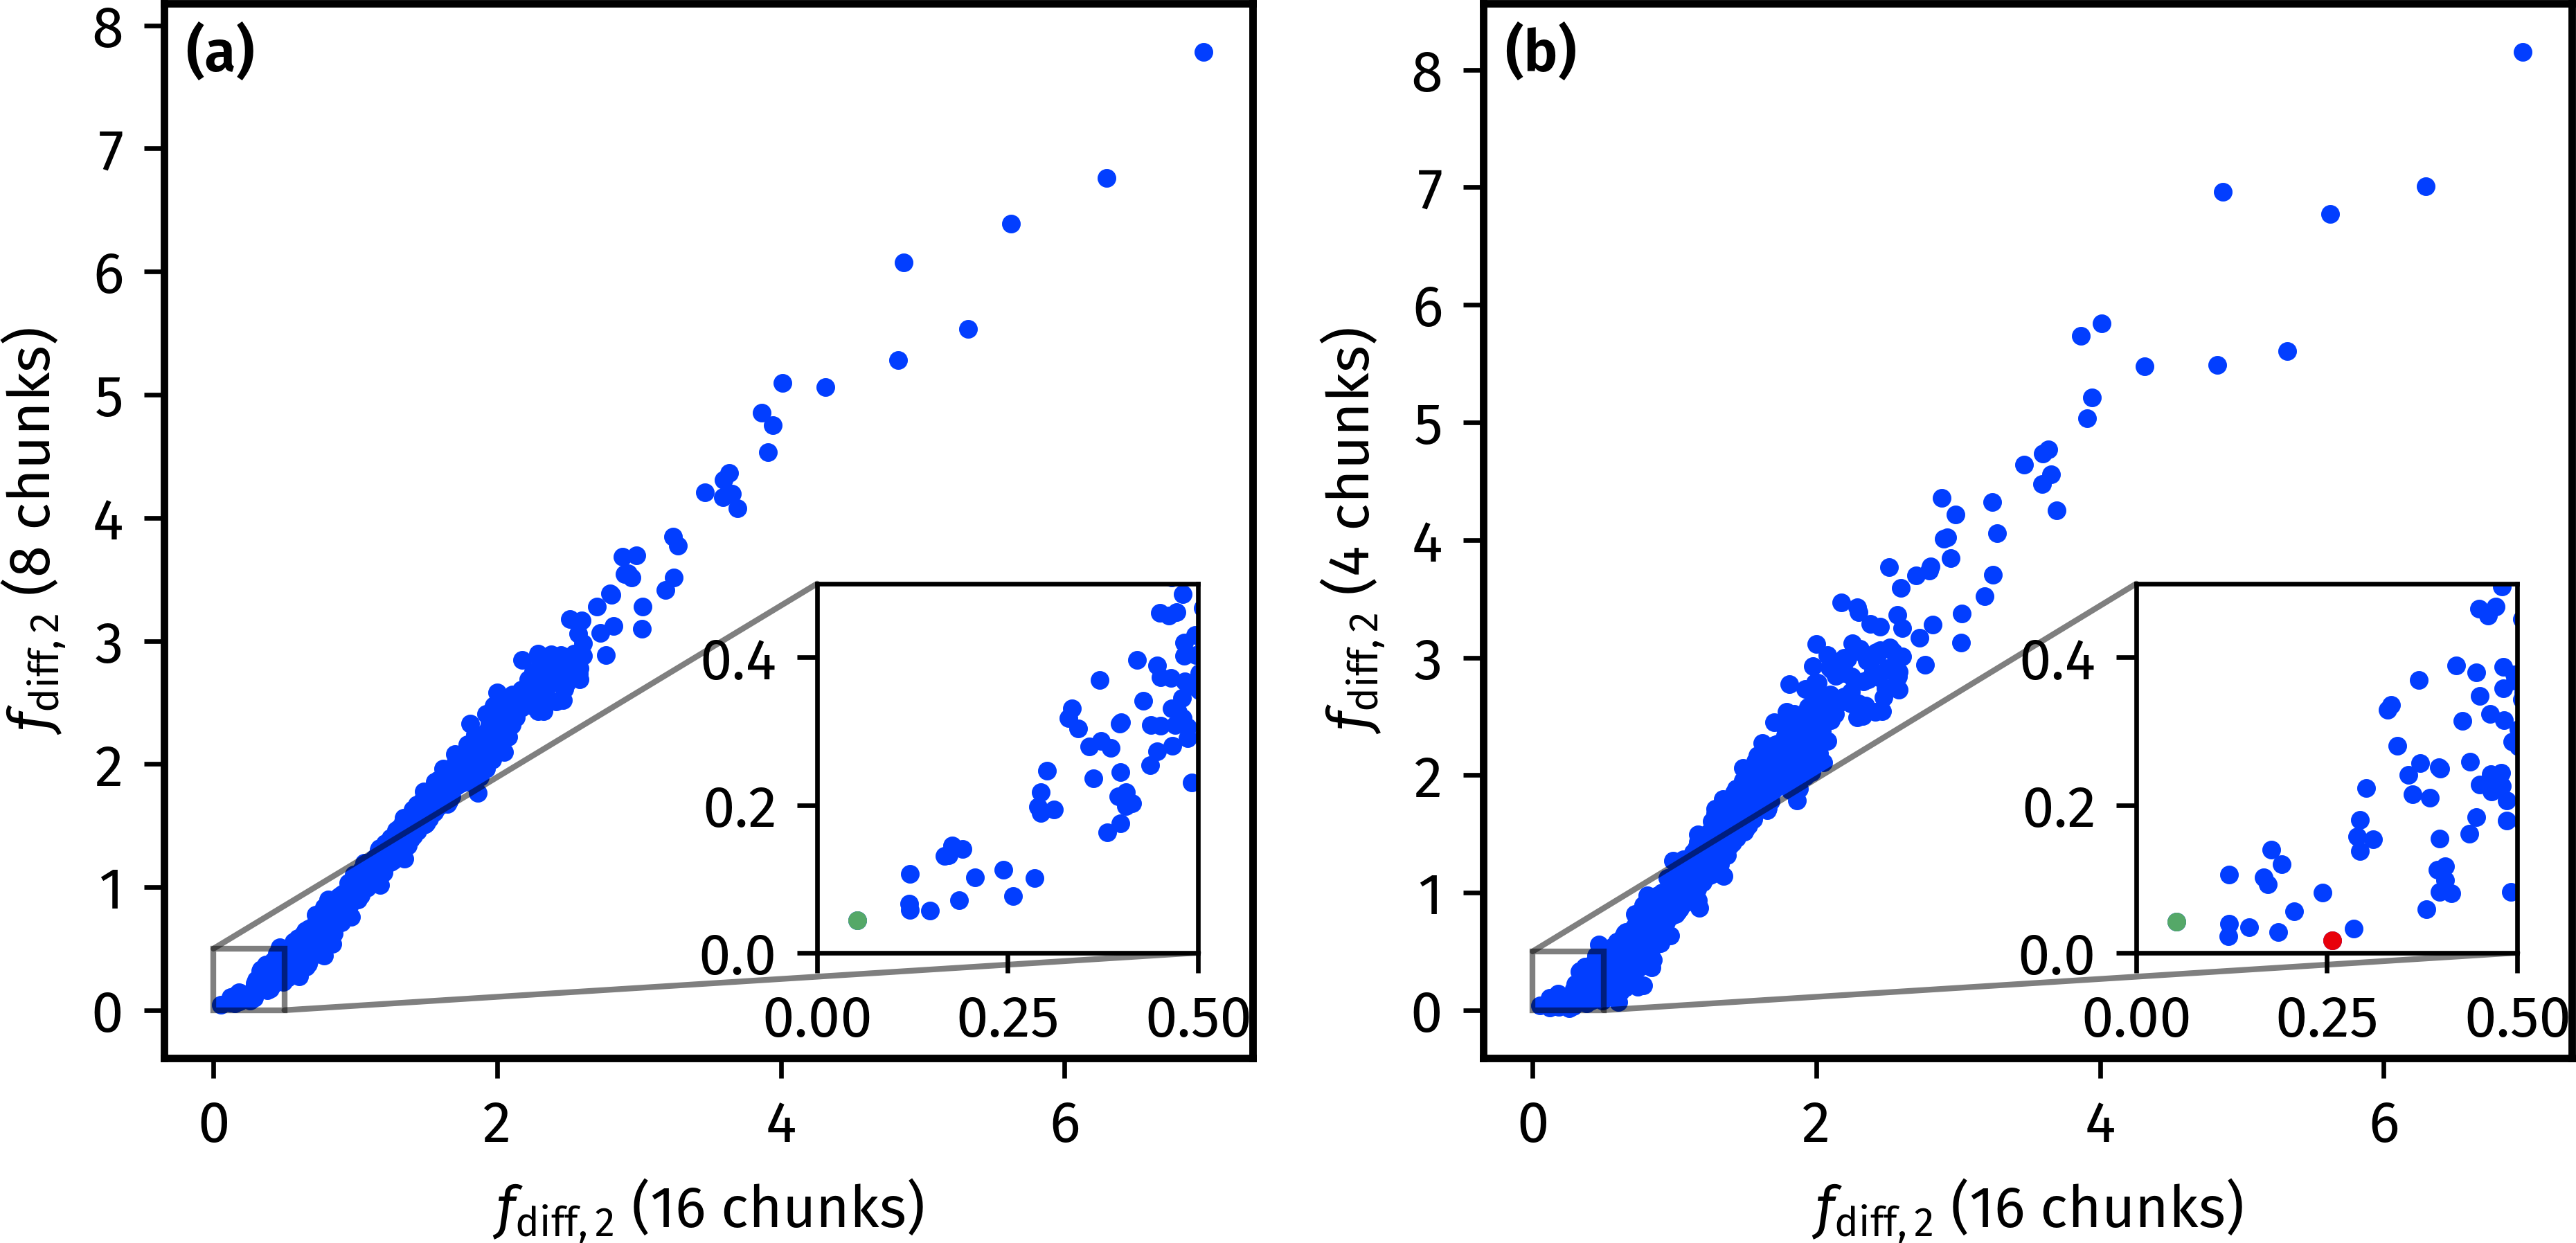
\includegraphics[]{pureshift/td1_cf.png}%
    {\phantomsubcaption\label{fig:dpsyche_td1_cf_16_8}}%
    {\phantomsubcaption\label{fig:dpsyche_td1_cf_16_4}}%
    \caption[Comparison of $f_\text{diff,2}$ cost function with different numbers of chunks]{
        Comparison of $f_\text{diff,2}$ values when simulated with different numbers of chunks.
        16 chunks is assumed to be the `gold standard'.
        \textbf{(\subref*{fig:dpsyche_td1_cf_16_8})} Correlation between 16-chunk and 8-chunk cost functions.
        The `optimum' identified by both cost functions is plotted in green in the inset.
        \textbf{(\subref*{fig:dpsyche_td1_cf_16_4})} Correlation between 16-chunk and 4-chunk cost functions.
        The `optima' identified by the 16- and 4-chunk cost functions are plotted in green and red respectively in the inset.
    }
    \label{fig:dpsyche_td1_cf}
\end{figure}

The 16-chunk and 8-chunk $f_\text{diff,2}$ (\cref{fig:dpsyche_td1_cf_16_8}) do in fact line up quite well.
Notably, as the inset shows, they both agree on the `best' candidate (note that this is not necessarily anywhere near perfect, since it was randomly generated).
The 4-chunk $f_\text{diff,2}$ also has the correct overall behaviour (\cref{fig:dpsyche_td1_cf_16_4}).
However, its ranking of the `best' candidates is not very accurate: the 4-chunk cost function rates the red dot in the inset as the optimum, but that is only the 13th-best candidate when using the 16-chunk cost function.
Ultimately, I decided to use the 4-chunk cost function for `quick and dirty' optimisations, where only an approximate optimum was required.
However, for anything requiring more accuracy, the 8-chunk cost function was used.

An optimisation was then carried out with a (rather arbitrarily chosen) setting of $m = 9$, i.e.\ nine hard pulses in the PSE.
A total of $s = 20$ spin systems were used, matching the number of CPU cores on the computer used for the optimisations: these were further subdivided into four two-spin systems, eight three-spin systems, and eight four-spin systems.
The derivative-based BFGS algorithm was used to carry out the optimisation: this is a popular line search algorithm which uses an approximate Hessian to calculate the search direction at each iteration.\autocite{Kelley1999,Nocedal2006}
No lower or upper bounds were placed on the flip angles or phases: phases can obviously simply be wrapped to the region $[0, 2\pi)$, and in the simulations, the hard pulses were modelled as being instantaneous rotations, so their flip angles can also just be wrapped to $[0, 2\pi)$.
(This would not be completely valid if realistic, finite pulses were used, since changing the flip angle would also change their duration.)
This first optimisation yielded the following optimised parameters for the nine pulses:
\begin{align}
    \{\beta_i\} &= \{\ang{118.6972}, \ang{29.8400}, \ang{107.4850}, \ang{190.4788}, \notag \\
                &\qquad \ang{138.4710}, \ang{144.5939}, \ang{18.9674}, \ang{73.8900}, \ang{130.6071}\} \label{eq:dpsyche_opt_nosens_angles} \\
     \{\phi_i\} &= \{\ang{144.5641}, \ang{173.3596}, \ang{38.9878}, \ang{146.3121}, \notag \\
                &\qquad \ang{127.7346}, \ang{7.5104}, \ang{36.9805}, \ang{110.2791}, \ang{182.3894}\}. \label{eq:dpsyche_opt_nosens_phases}
\end{align}
The fact that none of the flip angles exceeded \ang{360} here provides some justification for not using bounds in the optimisation.

\begin{figure}[htb]
    % I don't have the Matlab output data any more: it was done in
    % examples/run_opt_par() and predates some of the API rework to (e.g.)
    % enforce reproducibility. The angles and pulses are just taken from the
    % TopSpin data. :/ OK not ideal, I know, but too bad. Can't change it.
    % There IS one way to retrieve the data: rewind the entire git repo to this
    % date and rerun it.
    \centering
    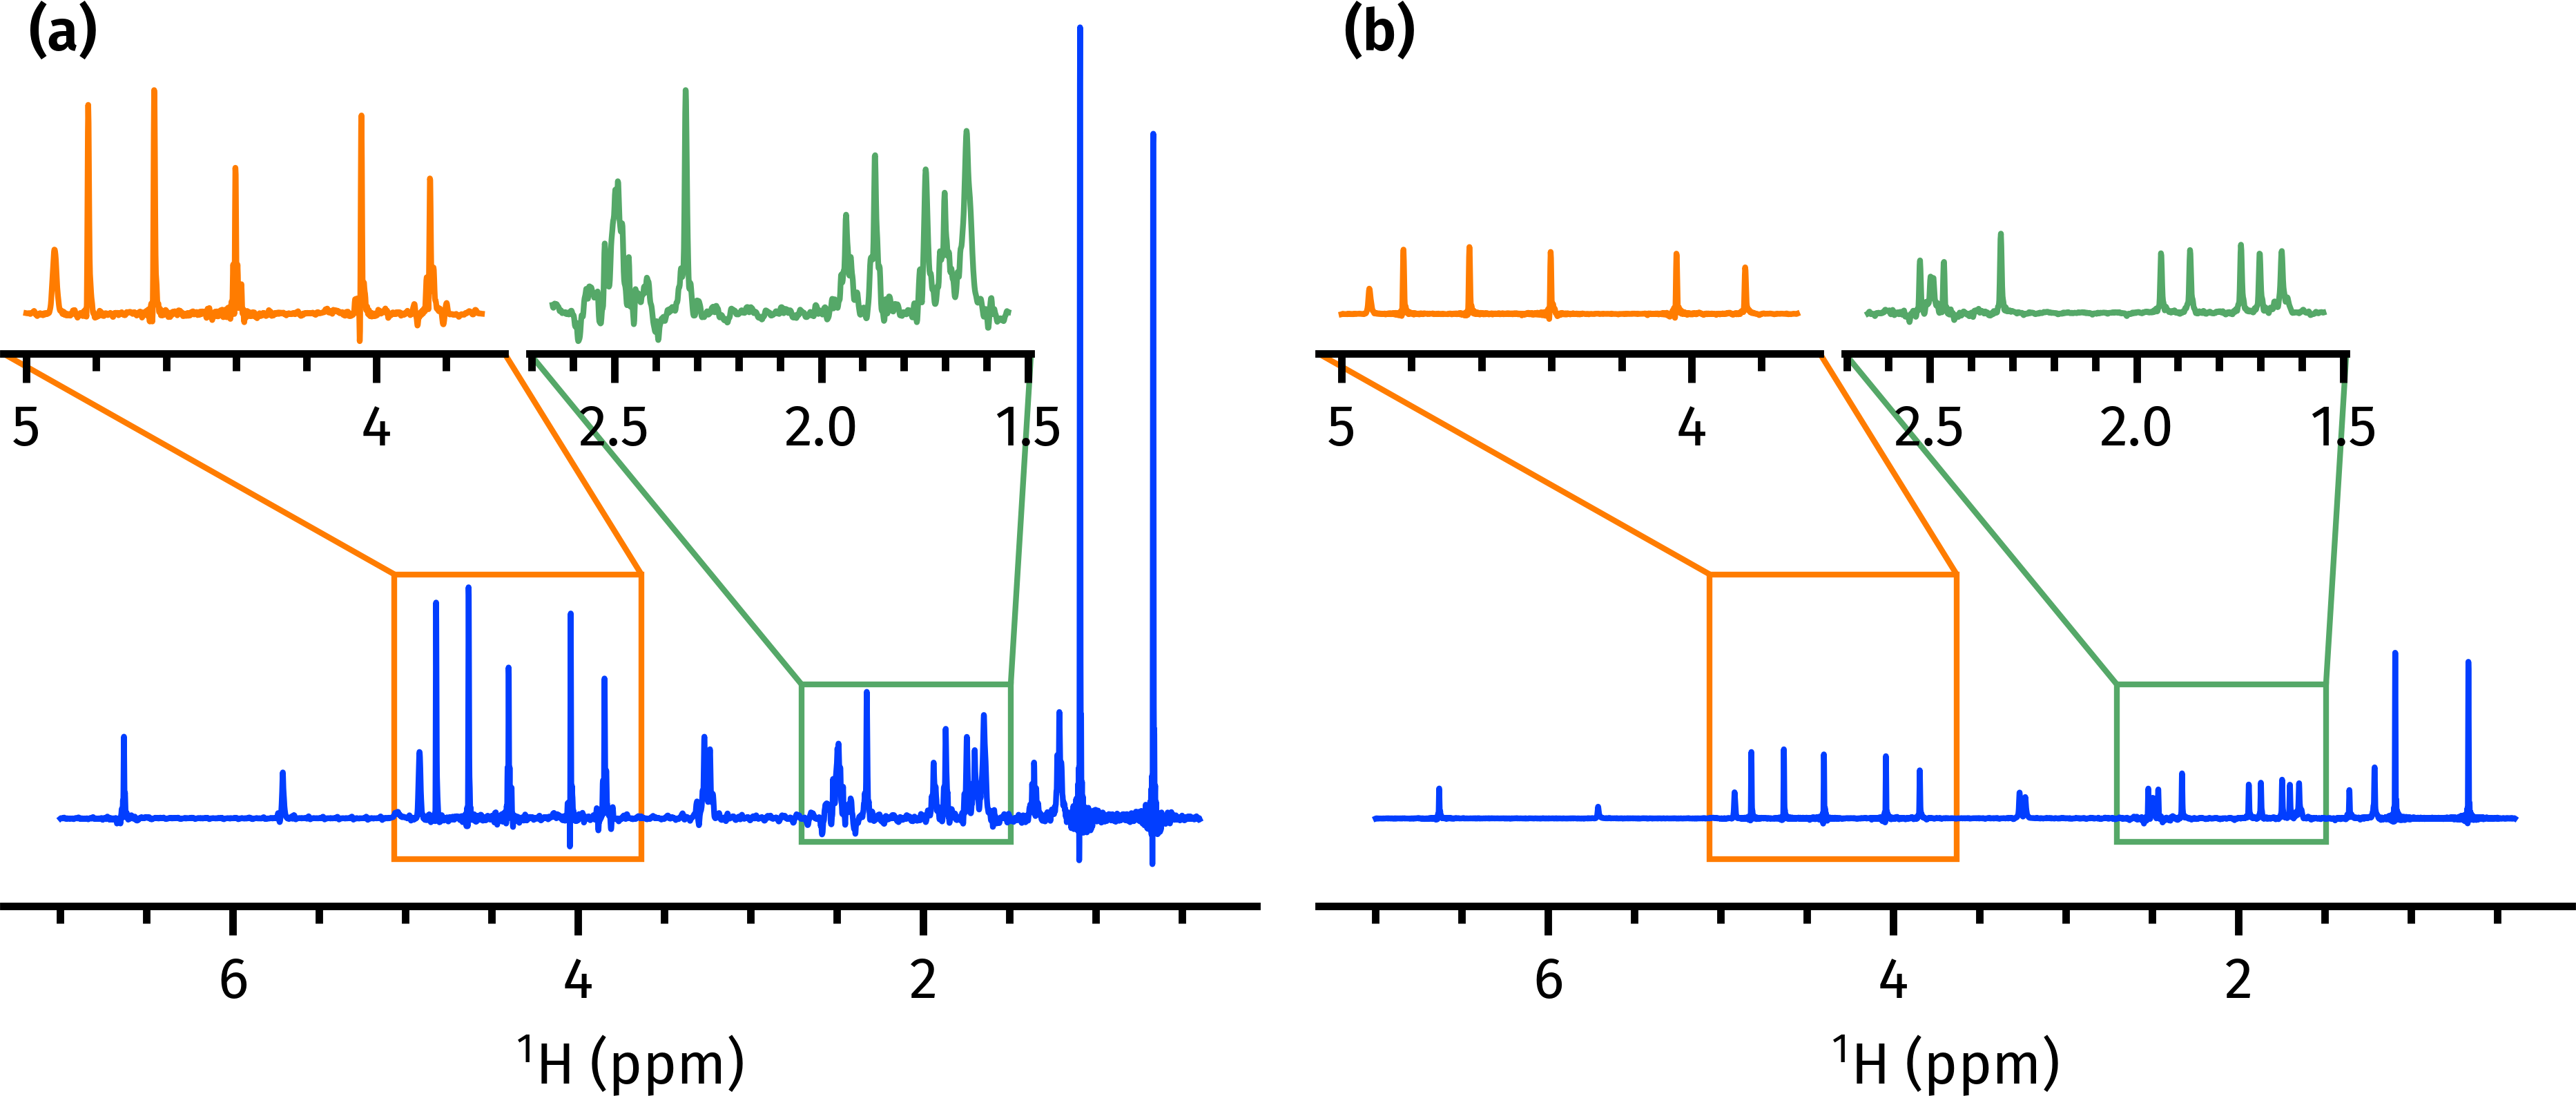
\includegraphics[]{pureshift/dpsyche_nosens_vs_psyche}%
    {\phantomsubcaption\label{fig:dpsyche_nosens_vs_psyche_dp}}%
    {\phantomsubcaption\label{fig:dpsyche_nosens_vs_psyche_p}}%
    \caption[Comparison of optimised dPSYCHE and PSYCHE]{
        \textbf{(\subref*{fig:dpsyche_nosens_vs_psyche_dp})} dPSYCHE experiment acquired using the flip angles and phases in \cref{eq:dpsyche_opt_nosens_angles,eq:dpsyche_opt_nosens_phases}.
        The $\beta$ hard pulses in the PSE were applied with an RF amplitude of 
        \textbf{(\subref*{fig:dpsyche_nosens_vs_psyche_p})} (Double-saltire) PSYCHE experiment acquired with $\beta = \ang{20}$.
        \datacode{6A-211027}
    }
    \label{fig:dpsyche_nosens_vs_psyche}
\end{figure}

To evaluate the quality of the decoupling on a real sample, the dPSYCHE experiment was performed experimentally, and the results compared against a PSYCHE experiment (\cref{fig:dpsyche_nosens_vs_psyche}).
Firstly, it is worth pointing out that a pure shift spectrum (even if not a very good one) was obtained: this validates the form of the PSE and the optimisation approach used here, especially considering that the optimisation was not tailored towards this particular sample.
The dPSYCHE experiment clearly has much greater sensitivity than the PSYCHE experiment; however, the decoupling quality is extremely poor.
The reason for this is likely because the optimisation is prioritising sensitivity too highly over purity, and ultimately stems from the factor $c$ in \cref{eq:f_diff_dpsyche} which we have ignored until now.
Since $c = 1$, the optimisation is essentially guiding the dPSYCHE experiment towards having \textit{exactly the same sensitivity as a pulse--acquire experiment}.

Although this might be a nice idea in principle, it is not physically sensible: no pure shift method has sensitivity which is even close to that of a pulse--acquire experiment.
It makes more sense to scale down the target spectrum by introducing a factor of $c < 1$ into the cost function (\cref{eq:f_diff_dpsyche}); the parameter $c$ therefore represents the `target sensitivity'.
By changing the parameter $c$, we can control whether the optimisation emphasises sensitivity or purity more.
(Note that this option was \textit{not} available to us in the experimental JRSE-based optimisations in \cref{sec:pureshift__optimisation}.)

A series of new optimisations were therefore run, with $c$ ranging from $0.2$ to $1$ (\cref{tbl:dpsyche_sens}).
The 4-chunk cost function was used, and the maximum number of function evaluations capped at 5000.
Each optimisation was run 10 times with a different starting seed, and the best of the 10 results chosen for further evaluation (\cref{tbl:dpsyche_sens}).
The resulting spectra (\cref{fig:dpsyche_sens}) show that adjusting $c$ has the desired effect: larger values lead to greater sensitivity and lower purity, and vice versa.

\begin{table}[htb]
    % matlab_nmr_jy/research/optim_specdiff/opt_sens.out
    \begin{tabular}{cccc}
        \toprule
        $c$ & \textbf{Flip angles} ($^\circ$) & \textbf{Phases} ($^\circ$) & $f_\text{diff,2}$ \\
        \midrule
        1 & \makecell{59.8813, 96.0748, 111.5862, \\ 118.7285, 144.701, 176.9773, \\ 29.2866, 40.0658, 63.8237} & \makecell{355.773, 81.741, 99.8752, \\ 81.6675, 337.0056, 150.7004, \\ 105.9666, 317.9979, 27.7897} & 0.0404 \\
        \midrule
        0.8 & \makecell{81.9461, 65.311, 90.3488, \\ 106.6388, 73.3462, 196.7857, \\ 51.791, 34.8188, 53.9506} & \makecell{329.8571, 60.3564, 137.3929, \\ 68.5286, 340.74, 126.29, \\ 64.4601, 145.4714, 27.3019} & 0.0321 \\
        \midrule
        0.6 & \makecell{53.1313, 82.2547, 88.6093, \\ 161.9291, 83.462, 161.3548, \\ 14.2976, 66.2199, 53.9709} & \makecell{347.2835, 59.5518, 68.072, \\ 113.5358, 34.5537, 156.191, \\ 268.7641, 302.7427, 16.29} & 0.0250 \\
        \midrule
        0.4 & \makecell{77.2998, 127.7274, 87.6663, \\ 104.6371, 99.6474, 168.8171, \\ 8.8569, 52.7865, 58.1408} & \makecell{342.2787, 47.7526, 76.4114, \\ 97.3304, 14.2178, 163.9513, \\ 94.2575, 280.0273, 16.0971} & 0.0271 \\
        \midrule
        0.2 & \makecell{120.6613, 107.6712, 84.0427, \\ 133.5377, 82.1999, 223.122, \\ 41.1617, 41.9398, 12.016} & \makecell{347.2051, 79.4503, 109.8796, \\ 83.5017, 345.4284, 133.8355, \\ 66.4118, 201.0041, 4.4419} & 0.0261 \\
        \midrule
        0.4* & \makecell{92.4395, 133.2136, 38.9704, \\ 34.9182, 56.0256, 57.4097, \\ 31.5916, 140.1088, 128.7125} & \makecell{62.036, 16.411, 319.5634, \\ 128.4443, 49.7357, 328.5103, \\ 210.6498, 44.0123, 327.4517} & 0.0108 \\
        \bottomrule
    \end{tabular}
    \caption[dPSYCHE optimisation results for different sensitivities]{
        Results of dPSYCHE optimisations for different sensitivities.
        Note that since the cost function depends on the value of $c$, the exact value of $f_\text{diff,2}$ for these optimisations cannot be compared to one another; they are only presented here for completeness.
        The final entry, labelled with an asterisk, was run with no limit on the number of function evaluations (this is discussed further in the text).
    }
    \label{tbl:dpsyche_sens}
\end{table}

\begin{figure}[htbp]
    % matlab_nmr_jy/research/optim_specdiff/opt_sens.m
    \centering
    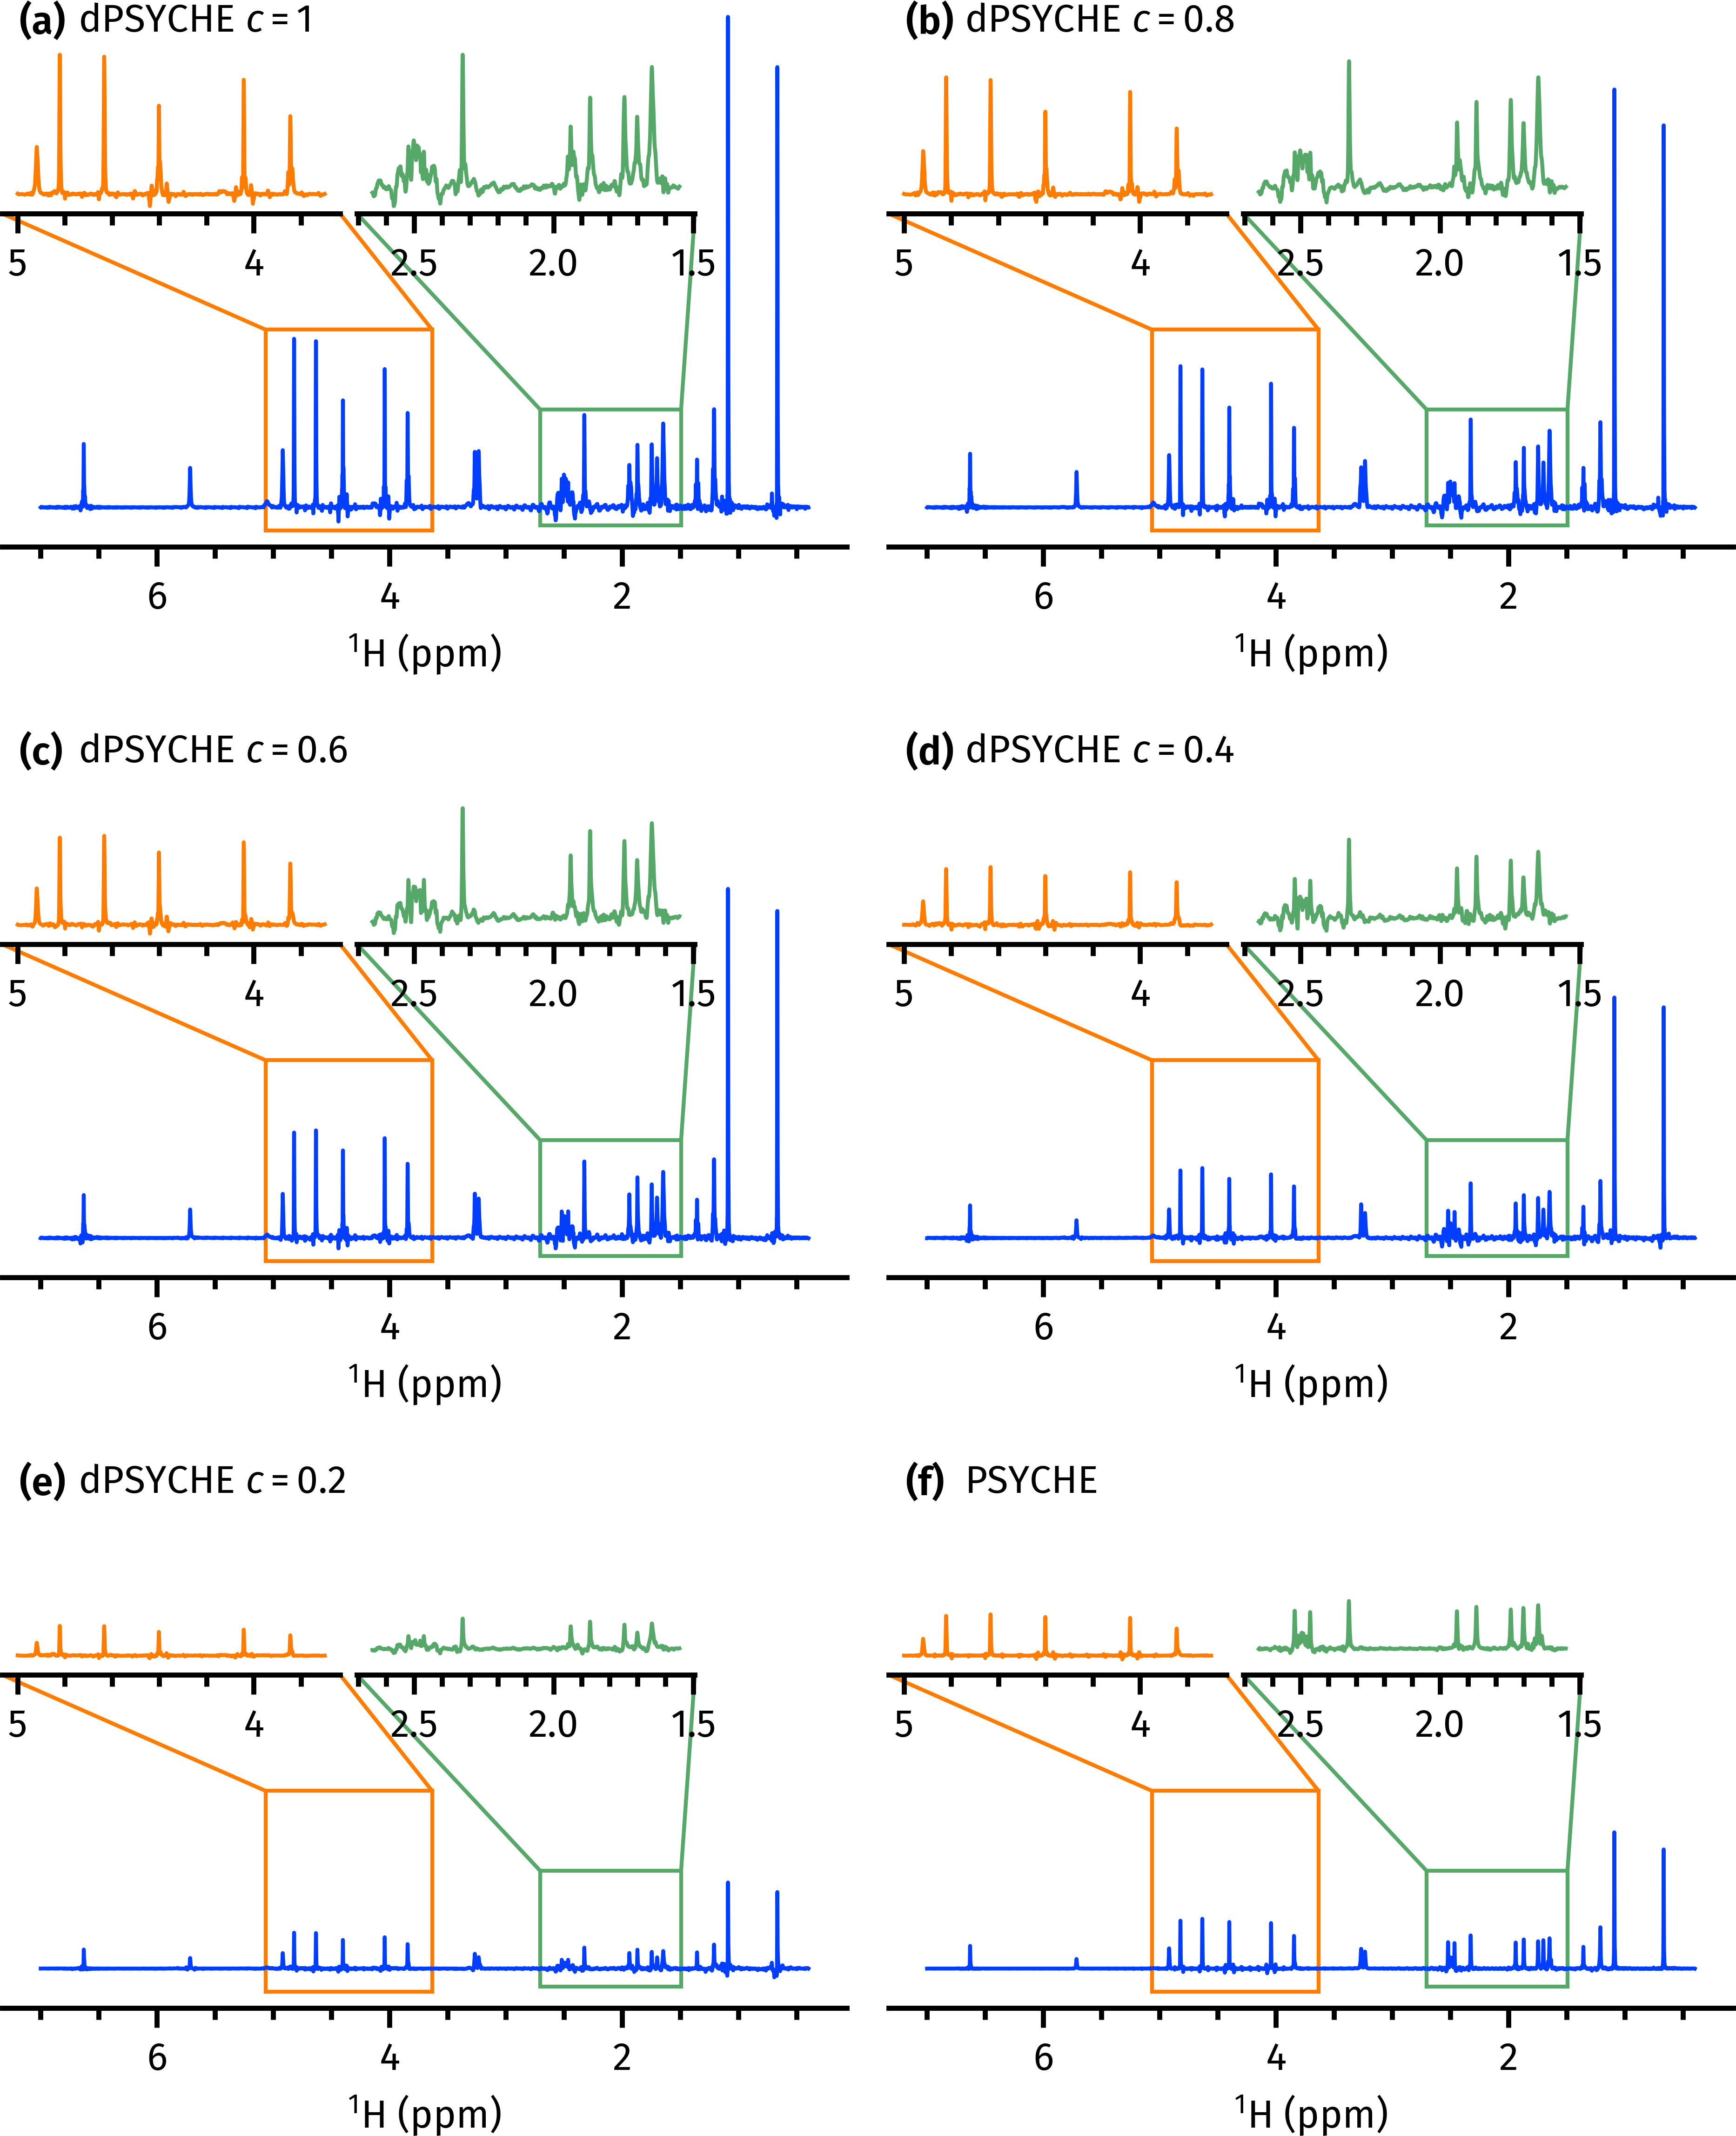
\includegraphics[]{pureshift/dpsyche_sens.png}%
    {\phantomsubcaption\label{fig:dpsyche_sens_d1}}%
    {\phantomsubcaption\label{fig:dpsyche_sens_d0p8}}%
    {\phantomsubcaption\label{fig:dpsyche_sens_d0p6}}%
    {\phantomsubcaption\label{fig:dpsyche_sens_d0p4}}%
    {\phantomsubcaption\label{fig:dpsyche_sens_d0p2}}%
    {\phantomsubcaption\label{fig:dpsyche_sens_p}}%
    \caption[dPSYCHE optimisations with different sensitivities]{
        \textbf{(\subref*{fig:dpsyche_sens_d1})} dPSYCHE, $c = 1$.
        \textbf{(\subref*{fig:dpsyche_sens_d0p8})} dPSYCHE, $c = 0.8$.
        \textbf{(\subref*{fig:dpsyche_sens_d0p6})} dPSYCHE, $c = 0.6$.
        \textbf{(\subref*{fig:dpsyche_sens_d0p4})} dPSYCHE, $c = 0.4$.
        \textbf{(\subref*{fig:dpsyche_sens_d0p2})} dPSYCHE, $c = 0.2$.
        \textbf{(\subref*{fig:dpsyche_sens_p})} Double-saltire PSYCHE with $\beta = \ang{20}$.
        All spectra and insets are plotted to scale to allow for sensitivity comparisons.
        \datacode{6A-211231}
    }
    \label{fig:dpsyche_sens}
\end{figure}

In this spectrum of andrographolide, the \qtyrange{3.5}{5}{\ppm} region (blue inset) is an `easier' region to decouple: there are fewer couplings here and all spin systems are firmly within the weak coupling regime.
The \qtyrange{1.5}{2.8}{\ppm} region (orange inset) is `more difficult' to decouple, especially the two peaks at \qty{2.5}{\ppm}, which are mutually strongly coupled.
The dPSYCHE spectrum with $c = 0.4$ appeared to be a good compromise between purity and sensitivity: its sensitivity was higher than that of the original (\ang{20} flip angle) PSYCHE experiment.
Furthermore, it provided good decoupling in the `easier' deshielded region and somewhat acceptable performance in the shielded region, with the notable exception of the strongly coupled peaks at \qty{2.5}{\ppm}.

I therefore ran a longer optimisation using the same starting point and with no limit on the number of function evaluations, which successfully lowered the cost function value by twofold (the last entry in \cref{tbl:dpsyche_sens}).
The pure shift spectrum obtained using these optimised pulses is shown in \cref{fig:dpsyche_optsens3}.
The decoupling quality in both regions is comparable to that in the PSYCHE spectrum, again with the exception of the strongly coupled peaks at \qty{2.5}{\ppm}.

\begin{figure}[htb]
    % matlab_nmr_jy/research/optim_specdiff/opt_sens3.m
    \centering
    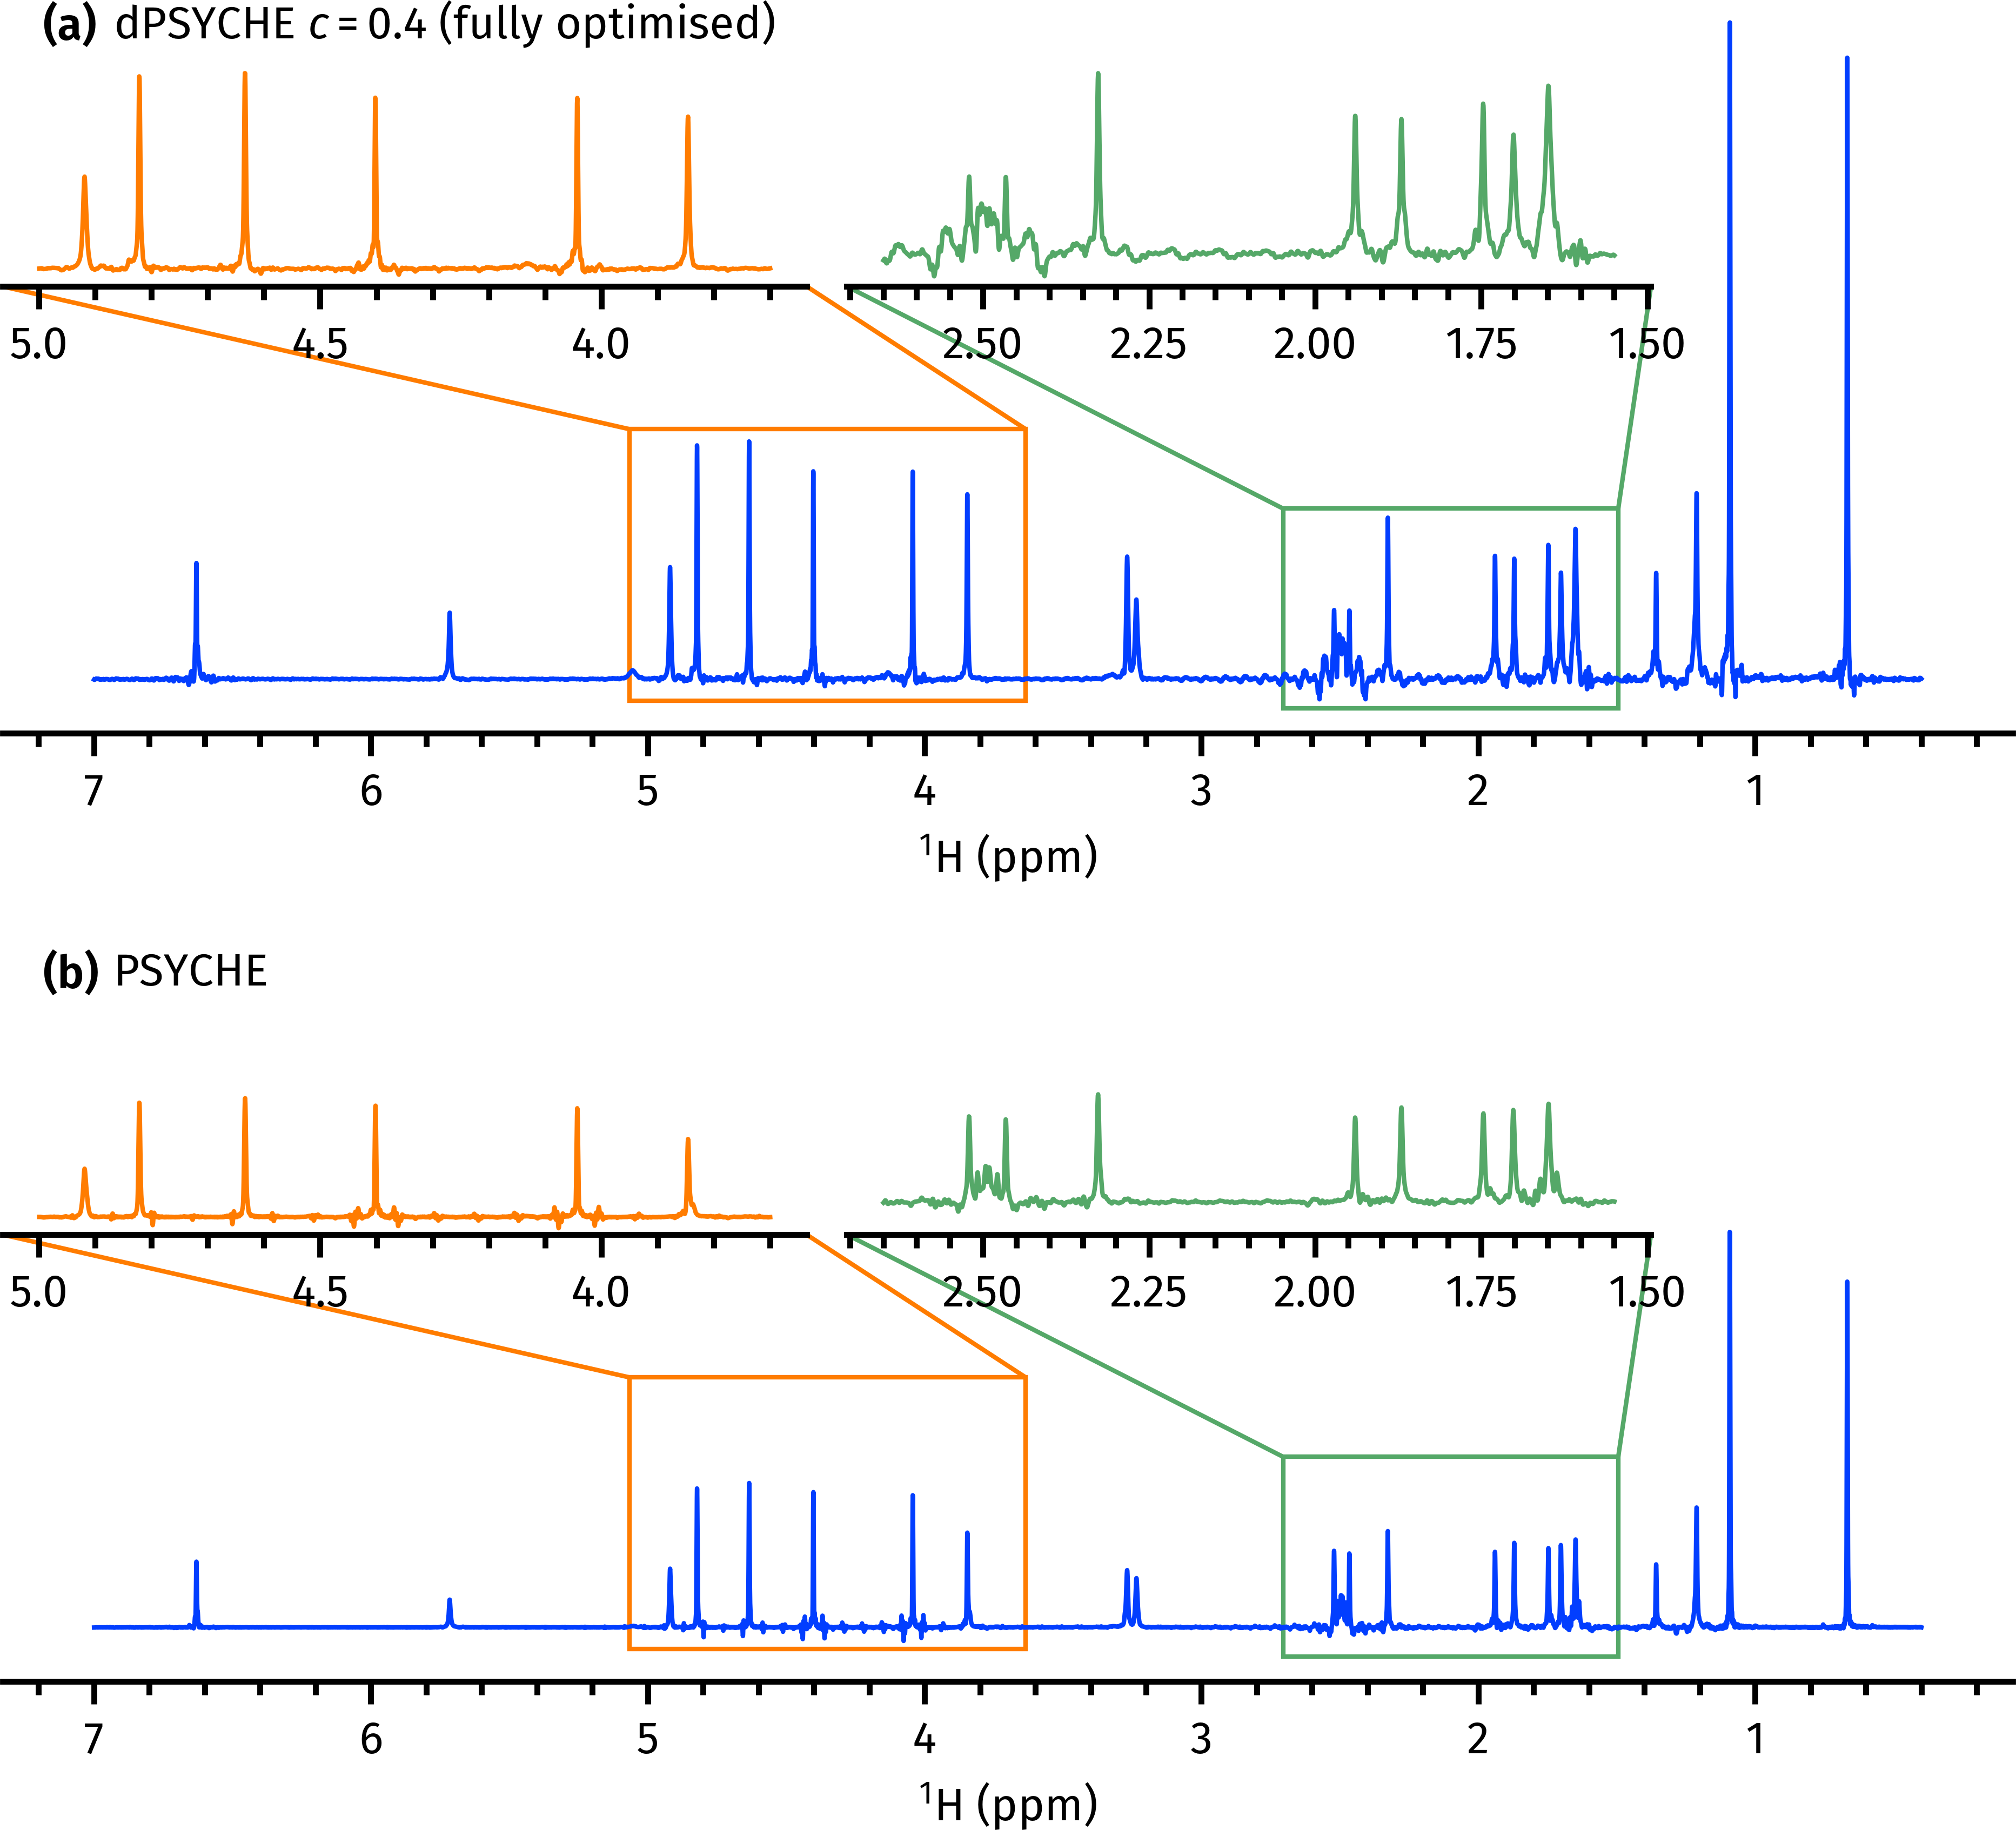
\includegraphics[]{pureshift/dpsyche_optsens3.png}%
    {\phantomsubcaption\label{fig:dpsyche_optsens3_d}}%
    {\phantomsubcaption\label{fig:dpsyche_optsens3_p}}%
    \caption[dPSYCHE final optimisation with $c = 0.4$]{
        \textbf{(\subref*{fig:dpsyche_optsens3_d})} Fully optimised dPSYCHE experiment with $c = 0.4$.
        \textbf{(\subref*{fig:dpsyche_optsens3_p})} Double-saltire PSYCHE with $\beta = \ang{20}$.
        \datacode{6A-211231}
    }
    \label{fig:dpsyche_optsens3}
\end{figure}

\begin{figure}[htb]
    % matlab_nmr_jy/research/optim_specdiff/opt_sens3.m but with different pulprog
    \centering
    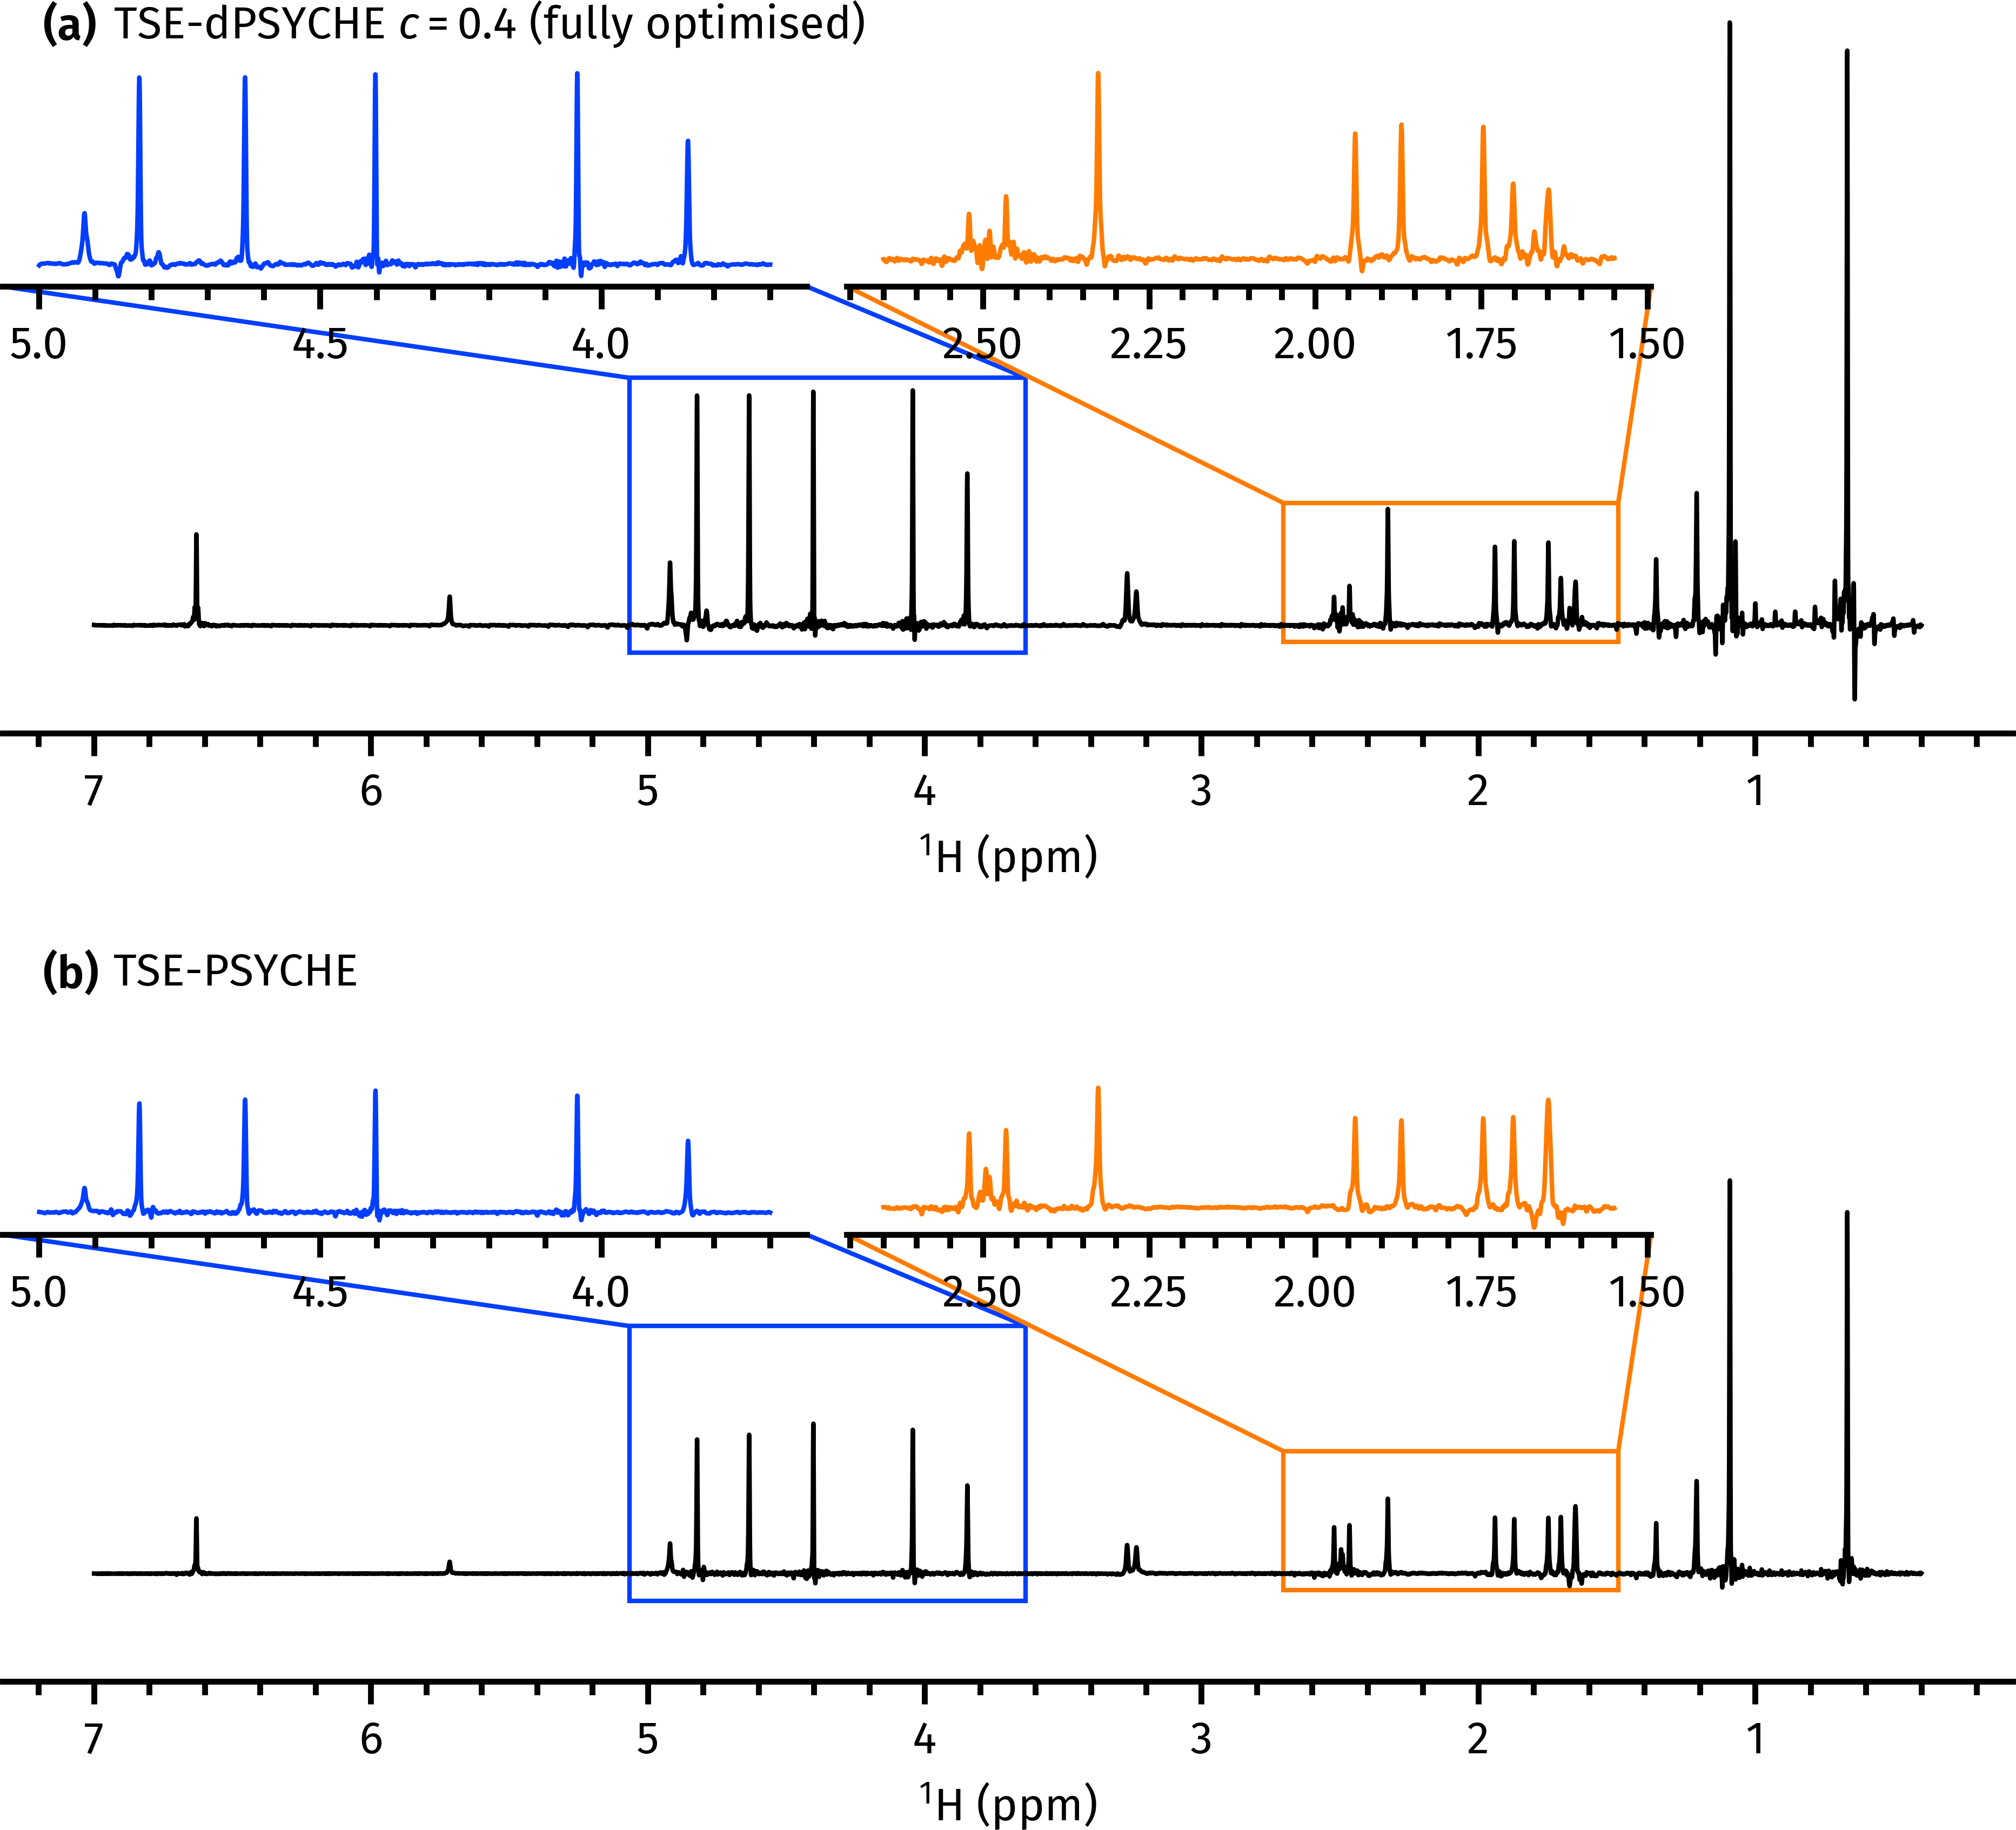
\includegraphics[]{pureshift/tsedpsyche_optsens3.png}%
    {\phantomsubcaption\label{fig:tsedpsyche_optsens3_d}}%
    {\phantomsubcaption\label{fig:tsedpsyche_optsens3_p}}%
    \caption[TSE-dPSYCHE final optimisation with $c = 0.4$]{
        \textbf{(\subref*{fig:tsedpsyche_optsens3_d})} Fully optimised TSE-dPSYCHE experiment with $c = 0.4$.
        \textbf{(\subref*{fig:tsedpsyche_optsens3_p})} Double-saltire TSE-PSYCHE with $\beta = \ang{20}$.
        \datacode{7A-220129}
    }
    \label{fig:tsedpsyche_optsens3}
\end{figure}

To make the dPSYCHE experiment more robust towards strong coupling, a TSE version of the sequence was also written and tested (\cref{fig:tsedpsyche_optsens3}).
This did indeed improve the decoupling at \qty{2.5}{\ppm}, as expected.
However, although the TSE-dPSYCHE version still retains its \textit{overall} sensitivity advantage over TSE-PSYCHE (especially evident in the deshielded region), this is not true of every peak: the two peaks at 1.65 and \qty{1.70}{\ppm} seem to have decreased intensities in the TSE-dPSYCHE experiment.
The reason for this is not fully clear.
One could say that the optimised pulses are not likely work equally well on \textit{all} combinations of chemical shifts and couplings, and these peaks may simply fall into one of the less effective regions; but in the (non-TSE) dPSYCHE experiment (\cref{fig:dpsyche_optsens3_d}), these distortions in intensity are not observed.
One possible conclusion is that some of the intensity in the non-TSE experiment in fact stems from artefacts which are not fully suppressed: this may also explain the slight broadening at the base of the peaks in \cref{fig:dpsyche_optsens3_d}.


% number of pulses (maybe can omit?)
\iffalse
I then ran several preliminary screens to decide on the number of pulses to include in the pulse sequence.
Here, the 8-chunk cost function was used.
To save time, the total number of function evaluations was capped at 600 times the number of pulses: this, together with the fact that only one optimisation per category was run, means that these results are more suggestive rather than conclusive.
(Since the BFGS algorithm is a local optimiser, and the trajectory depends quite strongly on the initial point, the optimisation should \textit{in theory} be run with several different initial points.)
There was no clear winner, but the optimisations with 9 and 15 pulses yielded the best results; since optimising 18 parameters is easier than 30, I opted to go with 9 pulses.

\begin{figure}[htb]
    \centering
    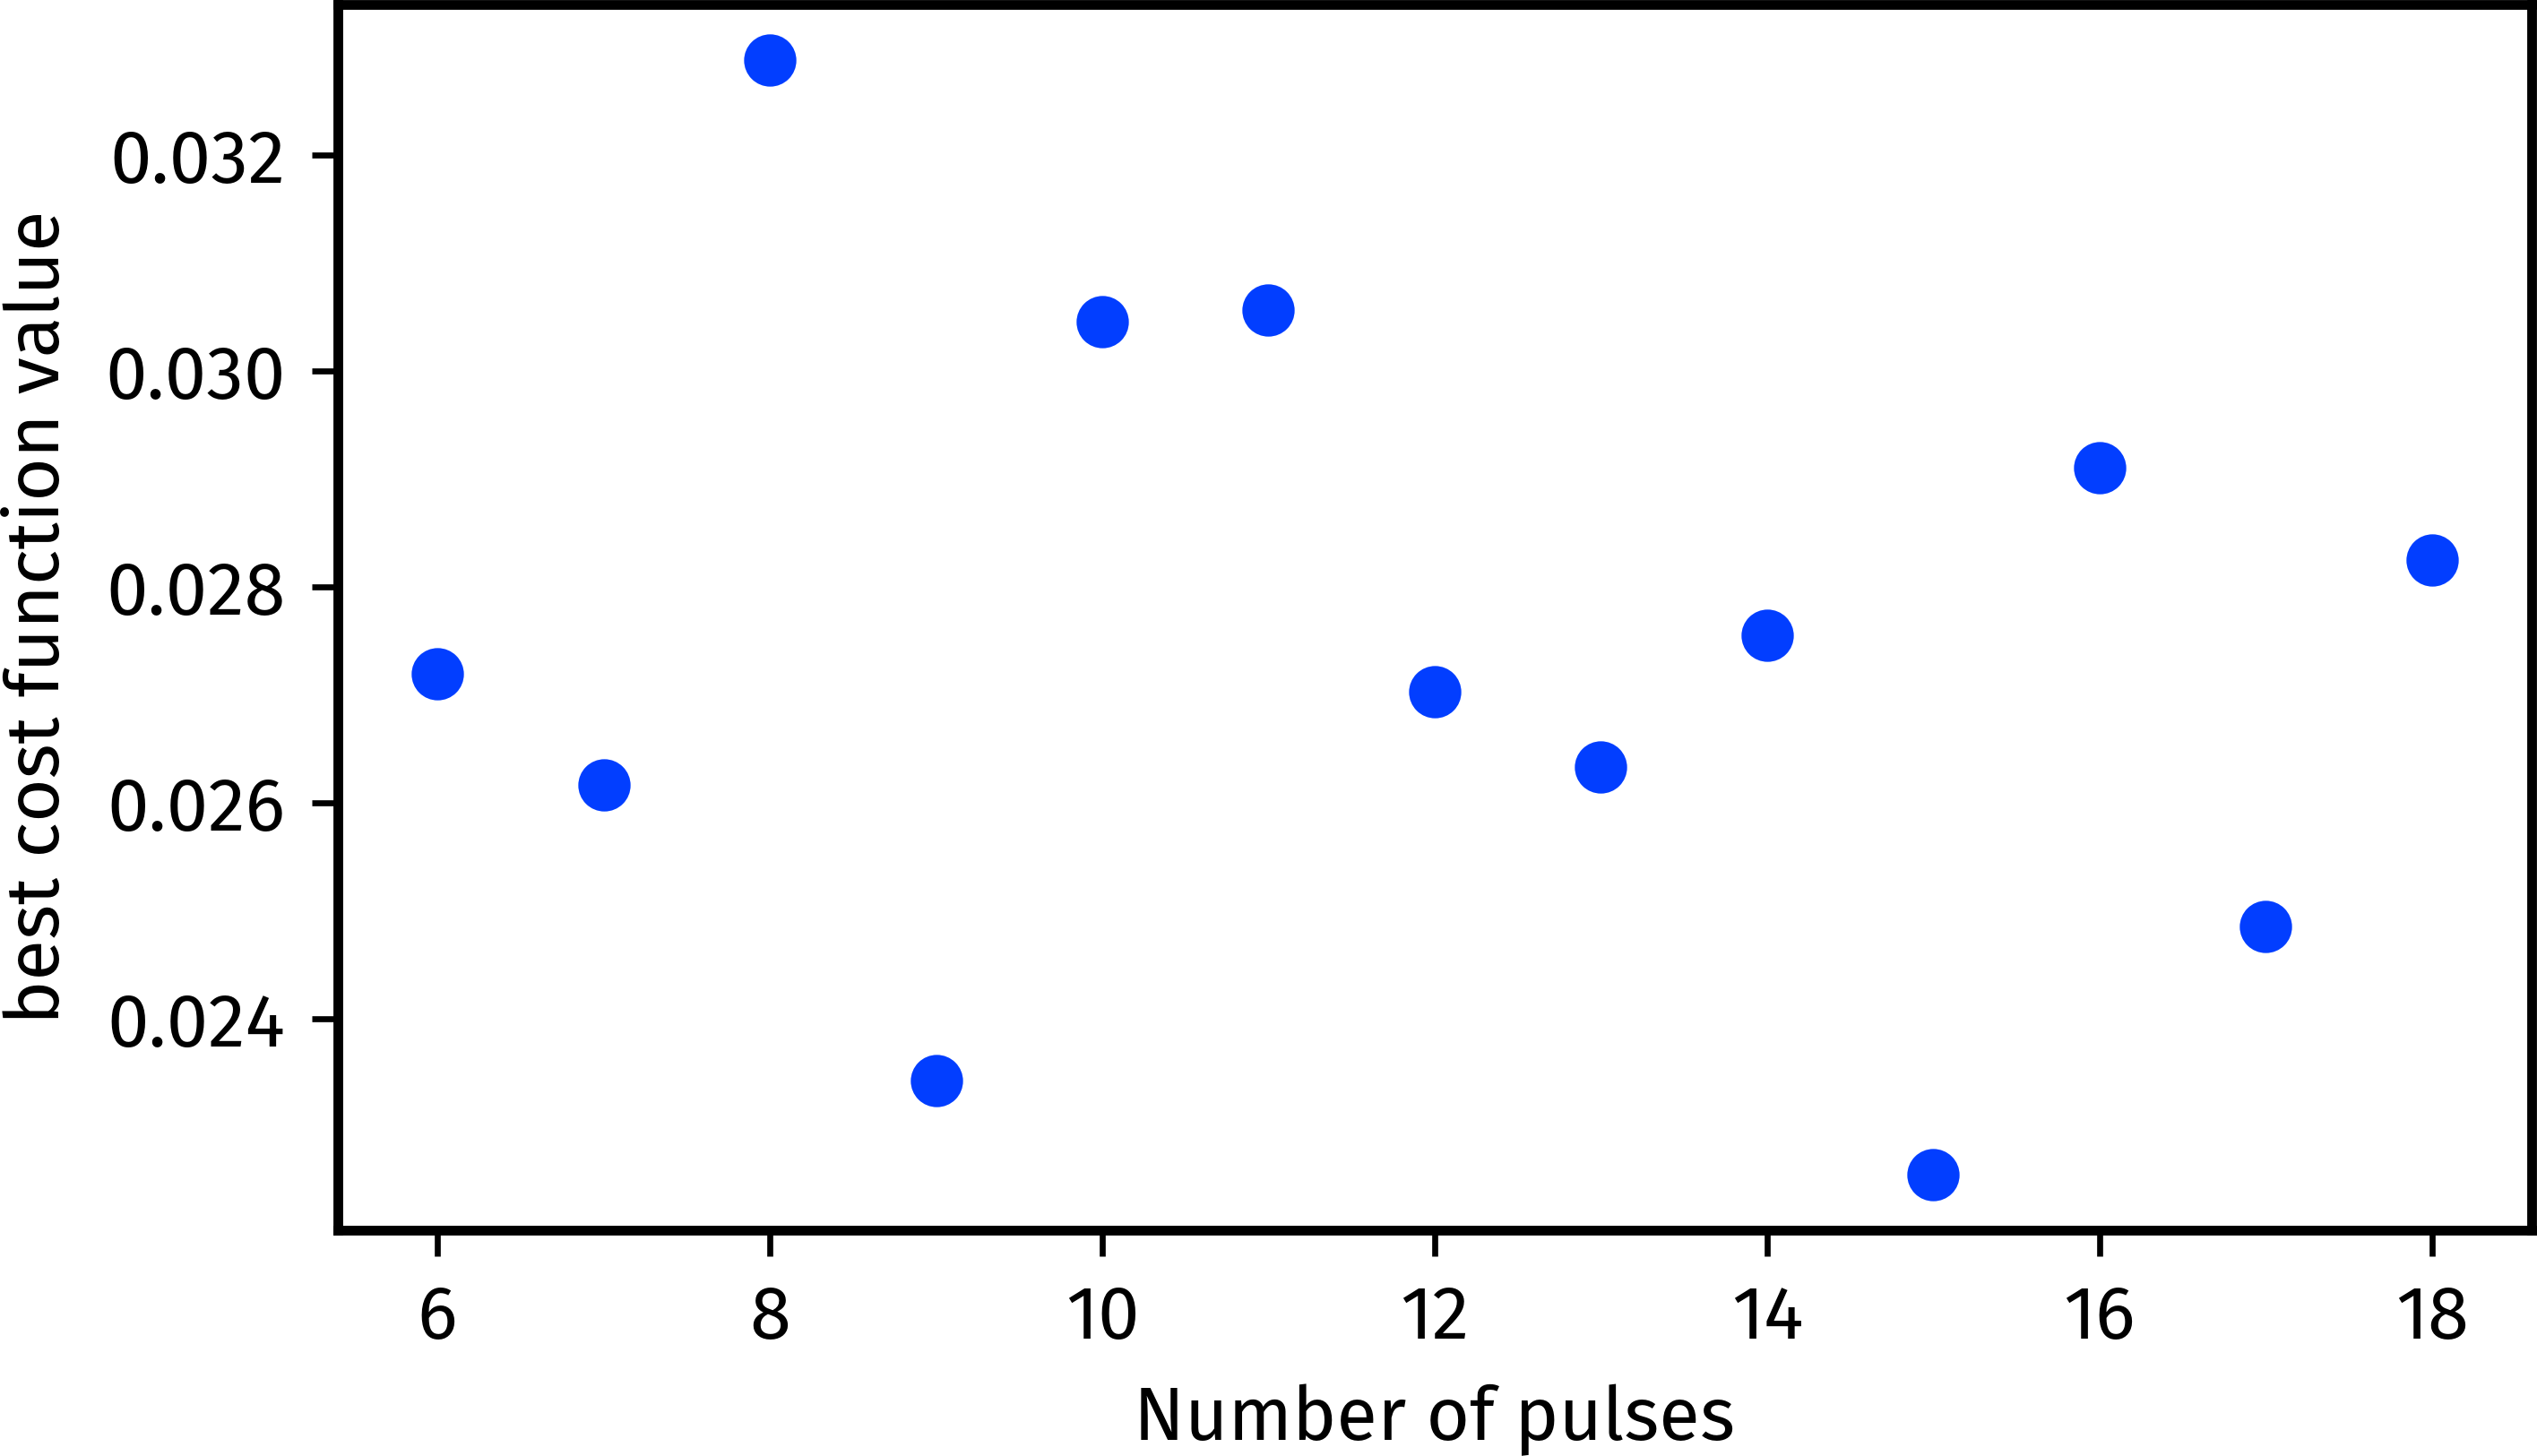
\includegraphics[]{pureshift/opt_npulses.png}%
    \caption[Comparison of cost functions attained with different numbers of pulses]{Blah}
    \label{fig:dpsyche_opt_npulses}
\end{figure}
\fi


\subsubsection{State-transfer cost function}

The optimisations conducted so far have been based on directly evaluating the simulated pure shift spectrum.
However, since these optimisations are conducted in a purely theoretical manner, it is possible to simply calculate the effect of the PSE on each input state to determine its quality.
We would want to maximise the degree of desired state transfer (which leads to the pure shift signal), and minimise the degree of unwanted state transfers (which lead to artefacts).
This would be a more direct way of evaluating the PSE.

We can split the possible state transfers up into several categories:
\begin{enumerate}
    \item desired (e.g.\ $I_{1+}I_{2\alpha} \to I_{1-}I_{2\alpha}$)
    \item undesired, but can be dephased by CTP gradients (e.g.\ $I_{1+}I_{2\alpha} \to I_{1+}I_{2\alpha}$)
    \item undesired, but can be suppressed by the TSE element (e.g.\ $I_{1+}I_{2\alpha} \to I_{1\alpha}I_{2-}$)
    \item undesired, but survive even with the TSE element (e.g.\ $I_{1+}I_{2\alpha} \to I_{1-}I_{2\beta}$)
\end{enumerate}
For a TSE-dPSYCHE experiment, we only need to consider items (1) and (4); without the TSE addition, we would additionally need to take item (3) into account.
These state transfer coefficients would also have to be summed over all possible input states: for an $n$-spin system, there are $n \cdot 2^{n-1}$ possible input states ($n$ possible spins which could be active, and $2^{n-1}$ permutations of passive spin states).
The cost function would then be constructed as a linear combination of these two or three terms, where the coefficients serve a similar function to the parameter $c$ in the spectrum-comparison cost function (\cref{eq:f_diff_dpsyche}) in that they control the balance between sensitivity and purity.

\todo{Table comparing fspec and fstate?}

Unfortunately, even though all of the code for efficient (parallelised) computation of this cost function was written, I did not have the time to actually perform optimisations using this cost function and to experimentally validate the results.
This is a slight disappointment to me, as the initial results shown in this section have been quite promising, and it is likely that the state transfer-based optimisations would have improved this even further.
However, even from just the results obtained so far, it is clear that the interleaved pulses and gradients used in the dPSYCHE PSE form a reasonable \textit{ansatz} which can yield pure shift spectra which are almost comparable to the PSYCHE method.
